\section{Methodology}
\frame{\tableofcontents[currentsection]}

\begin{frame}{Methodology overview}
    \begin{itemize}
        \item Feature extraction:
        \begin{itemize}
            \item Lexical features (32)
            \item Syntactic features (8)
            \item String features (18)
        \end{itemize}
        \vspace{0.4cm}
        \item Preprocessing: remove punctuation and convert to lower case.
        \begin{itemize}
            \item Extra preprocessing:
            \begin{itemize}
                \item Stop words (for lexical and string feature extraction)
                \item Lemmatization (for lexical and string feature extraction)
                \item Word sense disambiguation (for lexical feature extraction)
            \end{itemize}
        \end{itemize}
        \vspace{0.4cm}
        \item Training models:
        \begin{itemize}
            \item Multi-Layer Perceptron (MLP)
            \item Support Vector Regressor (SVR)
            \item Random Forest Regressor (RFR)
        \end{itemize} 
    \end{itemize}
\end{frame}


\begin{frame}{Lexical features}
    \textit{The process of analyzing a sentence's structure through the identification and classification of individual words.}
    \vspace{0.5cm}
    \begin{itemize}
        \item Jaccard distance 
        \item \textbf{Containtment similarity}
        \item \textbf{Pairwise word similarity}
        \item \textbf{Weighted word overlap}
        \item \textbf{WordNet augmented word overlap}
        \item \textbf{Greedy lemma aligning overlap}
    \end{itemize}
\end{frame}

    \begin{frame}{Lexical features}
        The sets $S_1$ and $S_2$ will be list of words or n-tuples of n-grams of each sentence. \\
        \begin{itemize}
            \item Containtment similarity measure (Broder, 1997)
            \[
            csimm(S_1,S_2) = \frac{\left| S_1 \cap S_2 \right|}{\min \{ \left| S_1 \right|, \left| S_2 \right| \}}
            \]
            \item Pairwise word similarity \\ 
            \begin{itemize}
                \item Mean of the maximum similarity using: Lin similarity and Resnik similarity weighted by Inverse Document Frequency (IDF) coefficient.

            \end{itemize}

            \item Weighted word overlap 
            \[
            wwc(S_1, S_2) = 
            \frac{\sum_{w \in S_1 \cap S_2} ic(w)}{\sum_{w' \in S_2} ic(w')}
            \]
        \end{itemize}
\end{frame}

\begin{frame}{Lexical features}
    \begin{itemize}
    \item WordNet augmented word overlap 
    \[ P_{WN}(S_1, S_2) = \frac{1}{|S_2|} \sum_{w_1 \in S_1} \text{score}(w_1, S_2)\]
    \[
    \text{score}(w, S) = 
    \begin{cases} 
    1 & \text{if } w \in S \\ 
    \max_{w' \in S} \{\text{pathsim}(w, w')\} & \text{otherwise}
    \end{cases}
    \]
    \vspace{0.3cm}
\item Greedy lemma aligning overlap
    \[ glao(S_1, S_2) = \frac{\sum_{(l_1, l_2) \in P} \max \{ \text{ic}(l_1), \text{ic}(l_2) \} \cdot \text{linsim}(l_1, l_2)}{\max \{|S_1|, |S_2|\}} \]
    P is the set of lemma pairs obtained by greedy alignment.
\end{itemize}
\end{frame}

\begin{frame}{Syntactic Features}
    \textit{Process of analyzing a sentence's structure according to the grammatical rules and how words are related within
    the sentence.}
    \vspace{1cm}
    \begin{itemize}
        \item N-grams overlap removing function words (prepositions, conjunctions, articles)
    \end{itemize}
    \vspace{1cm}
    Sentence: "a horse eats carrots" $\Rightarrow$ "horse eats carrots" (content words)
         \[ ngo(S_1, S_2) = 2 \cdot \left( \frac{|S_1|}{|S_1 \cap S_2|} + \frac{|S_2|}{|S_1 \cap S_2|} \right)^{-1} \]
\end{frame}

\begin{frame}{Syntactic Features}
    \begin{itemize}
        \item Syntactic roles similarity 
    \end{itemize}
    \vspace{0.3cm}
    \texttt{python library Stanza} (Stanford NLP Group, 2006)\\ \vspace{0.1cm}
    Sentence: "a horse eats carrots and the man cleans the farm for the owner" \\ \vspace{0.1cm}
    \texttt{'p': [\{'carrot','eat'\}, \{'owner','farm','for','clean'\}],
    \\ 's': [\{'horse'\}, \{'man'\}], 
    \\ 'o': [\{'carrot'\}, \{'farm'\}, \{'for', 'owner'\}]}
         \[ chunksim(C1, C2) = \sum_{ l_1 \in C1} \sum_{l_2 \in C2}  ssim(l_1, l_2) \]
\end{frame}

\begin{frame}{Syntactic Features}
    \begin{itemize}
        \item Syntactic dependencies overlap
    \end{itemize}
    \vspace{0.2cm}
    \texttt{python library Stanza} (Stanford NLP Group, 2006) \\
    Sentence: "a horse eats carrots" \\
    \begin{center}
        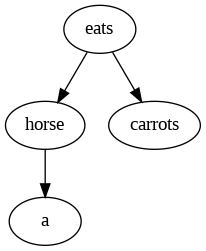
\includegraphics[width=0.22\textwidth]{figures/dependency_tree.png}
    \end{center}
        \[ \text{wdrc}(S_1, S_2) = \frac{\sum_{r \in S_1 \cap S_2} \max(\text{ic}(g(r)), \text{ic}(d(r)))}{\sum_{r \in S_2} 
\max(\text{ic}(g(r)), \text{ic}(d(r)))} \]
\end{frame}


\begin{frame}{String Feature}

    \begin{itemize}
        \item Character n-grams (Barrón-Cedeño, 2010)
        \vspace{0.2cm}
        \begin{itemize}
            \item \texttt{from sklearn.feature\_extraction.text import TfidfVectorizer} 
        \end{itemize}
        \vspace{0.2cm} 
        Sentece: "a horse eats carrots" \\ \vspace{0.2cm}
        3-grams strigns: ['a h', ' ho', 'hor', 'ors', 'rse', 'se ', 'e e', ' ea', 'eat', 'ats', 'ts ', 's c', ' ca', 'car', 'arr', 'rro', 'rot', 'ots']
        \[ 
            \text{cossim(A,B)} = \frac{\mathbf{A} \cdot \mathbf{B}}{\|\mathbf{A}\| \|\mathbf{B}\|}
             \]
    \end{itemize}

    \begin{itemize}
        \item Greedy String Tiling
    \end{itemize}
    \[
gstsim(S_1, S_2) = \frac{\sum_{t \in S_1 \cap S_2} \text{len}(t)}{\max \{ \text{len}(S_1), \text{len}(S_2) \}}
\]
        Threshold for the lenght of the tile: 5, 10. \\ \vspace{0.1cm}
\end{frame}
